\documentclass[tikz]{standalone}
\usepackage{tikz}
\usetikzlibrary{positioning, shapes.multipart, arrows, shadows, backgrounds, fit}
\usepackage{amsmath}
\usepackage{amssymb}
\usepackage{amsthm}

\tikzset{
	WL/.style={
		draw,
		rectangle,
		minimum height=2.4cm,
		text width = .15cm,
		fill=cyan,
		align=center,
		inner sep=2ex
	},
}
\usetikzlibrary{decorations.shapes}
\newcommand{\fillcolor}{cyan!70!black}
\newcommand{\fillcolorgreen}{green!70!black}
\newcommand{\fillcoloblue}{blue!70!black}
\newcommand{\boundarycolor}{black}
\tikzset{decorate sep/.style 2 args=
	{decorate,decoration={shape backgrounds,shape=circle,shape size=#1,shape sep=#2}}}


\usetikzlibrary{fadings,shapes.arrows,shadows}   
\usetikzlibrary{calc,tikzmark}

\newcommand{\vc}[1]{{\color{magenta!80!black}#1}}
\newcommand{\wc}[1]{{\color{blue}#1}}
\renewcommand{\d}{\text{\sffamily{d}}}

\tikzfading[name=arrowfading, top color=transparent!0, bottom color=transparent!95]
\tikzset{arrowfill/.style={top color= black!20, bottom color=black, text= white, general shadow={fill=black, shadow yshift=-0.8ex, path fading=arrowfading}}}

\tikzset{arrowstyle/.style={draw=black,arrowfill, single arrow,minimum height=#1, single arrow,
		single arrow head extend=.4cm,}}

\tikzset{arrowstylesecond/.style={draw=black,arrowfill, double arrow,minimum height=#1, double arrow,
		double arrow head extend=.4cm,}}
	
\newcommand{\tikzfancyarrow}[2][2cm]{\tikz[baseline=-0.5ex]\node [arrowstyle=#1] {#2};}
\newcommand{\tikzfancyarrowsecond}[2][2cm]{\tikz[baseline=-0.5ex]\node [arrowstylesecond=#1] {#2};}

\newcommand{\rk}{{\sffamily{RK4}}}

\usepackage{color}
\definecolor{bluegreen}{rgb}{0.0, 0.87, 0.87}
\usetikzlibrary{fadings,shapes.arrows,shadows}   
\usetikzlibrary{shapes.multipart}

\tikzfading[name=arrowfading, top color=transparent!0, bottom color=transparent!95]
\tikzset{arrowfill/.style={top color= black!20, bottom color=orange, general shadow={fill=black, shadow yshift=-0.8ex, path fading=arrowfading}}}
\tikzset{arrowstyle/.style={draw=black,arrowfill, single arrow,minimum height=#1, single arrow,
		single arrow head extend=.4cm,}}

\usetikzlibrary{decorations.pathreplacing,calligraphy}

%% https://tex.stackexchange.com/questions/55068/is-there-a-tikz-equivalent-to-the-pstricks-ncbar-command
\tikzset{
	ncbar angle/.initial=90,
	ncbar/.style={
		to path=(\tikztostart)
		-- ($(\tikztostart)!#1!\pgfkeysvalueof{/tikz/ncbar angle}:(\tikztotarget)$)
		-- ($(\tikztotarget)!($(\tikztostart)!#1!\pgfkeysvalueof{/tikz/ncbar angle}:(\tikztotarget)$)!\pgfkeysvalueof{/tikz/ncbar angle}:(\tikztostart)$)
		-- (\tikztotarget)
	},
	ncbar/.default=0.5cm,
}

\tikzset{square left brace/.style={ncbar=0.5cm}}
\tikzset{square right brace/.style={ncbar=-0.5cm}}

\tikzset{round left paren/.style={ncbar=0.5cm,out=120,in=-120}}
\tikzset{round right paren/.style={ncbar=0.5cm,out=60,in=-60}}


\begin{document}
	\tikzstyle{sum} = [draw = red!50!black, fill=cyan, circle=.1cm, node distance=.5cm]
	\begin{tikzpicture}[font=\sffamily]
		\node[ fill = white,draw = green!50!black, text = black, thick,rounded corners = 0.5ex] (burger) {\begin{tabular}{c}
				{\color{red!30!black} \huge Dataset}  \\ 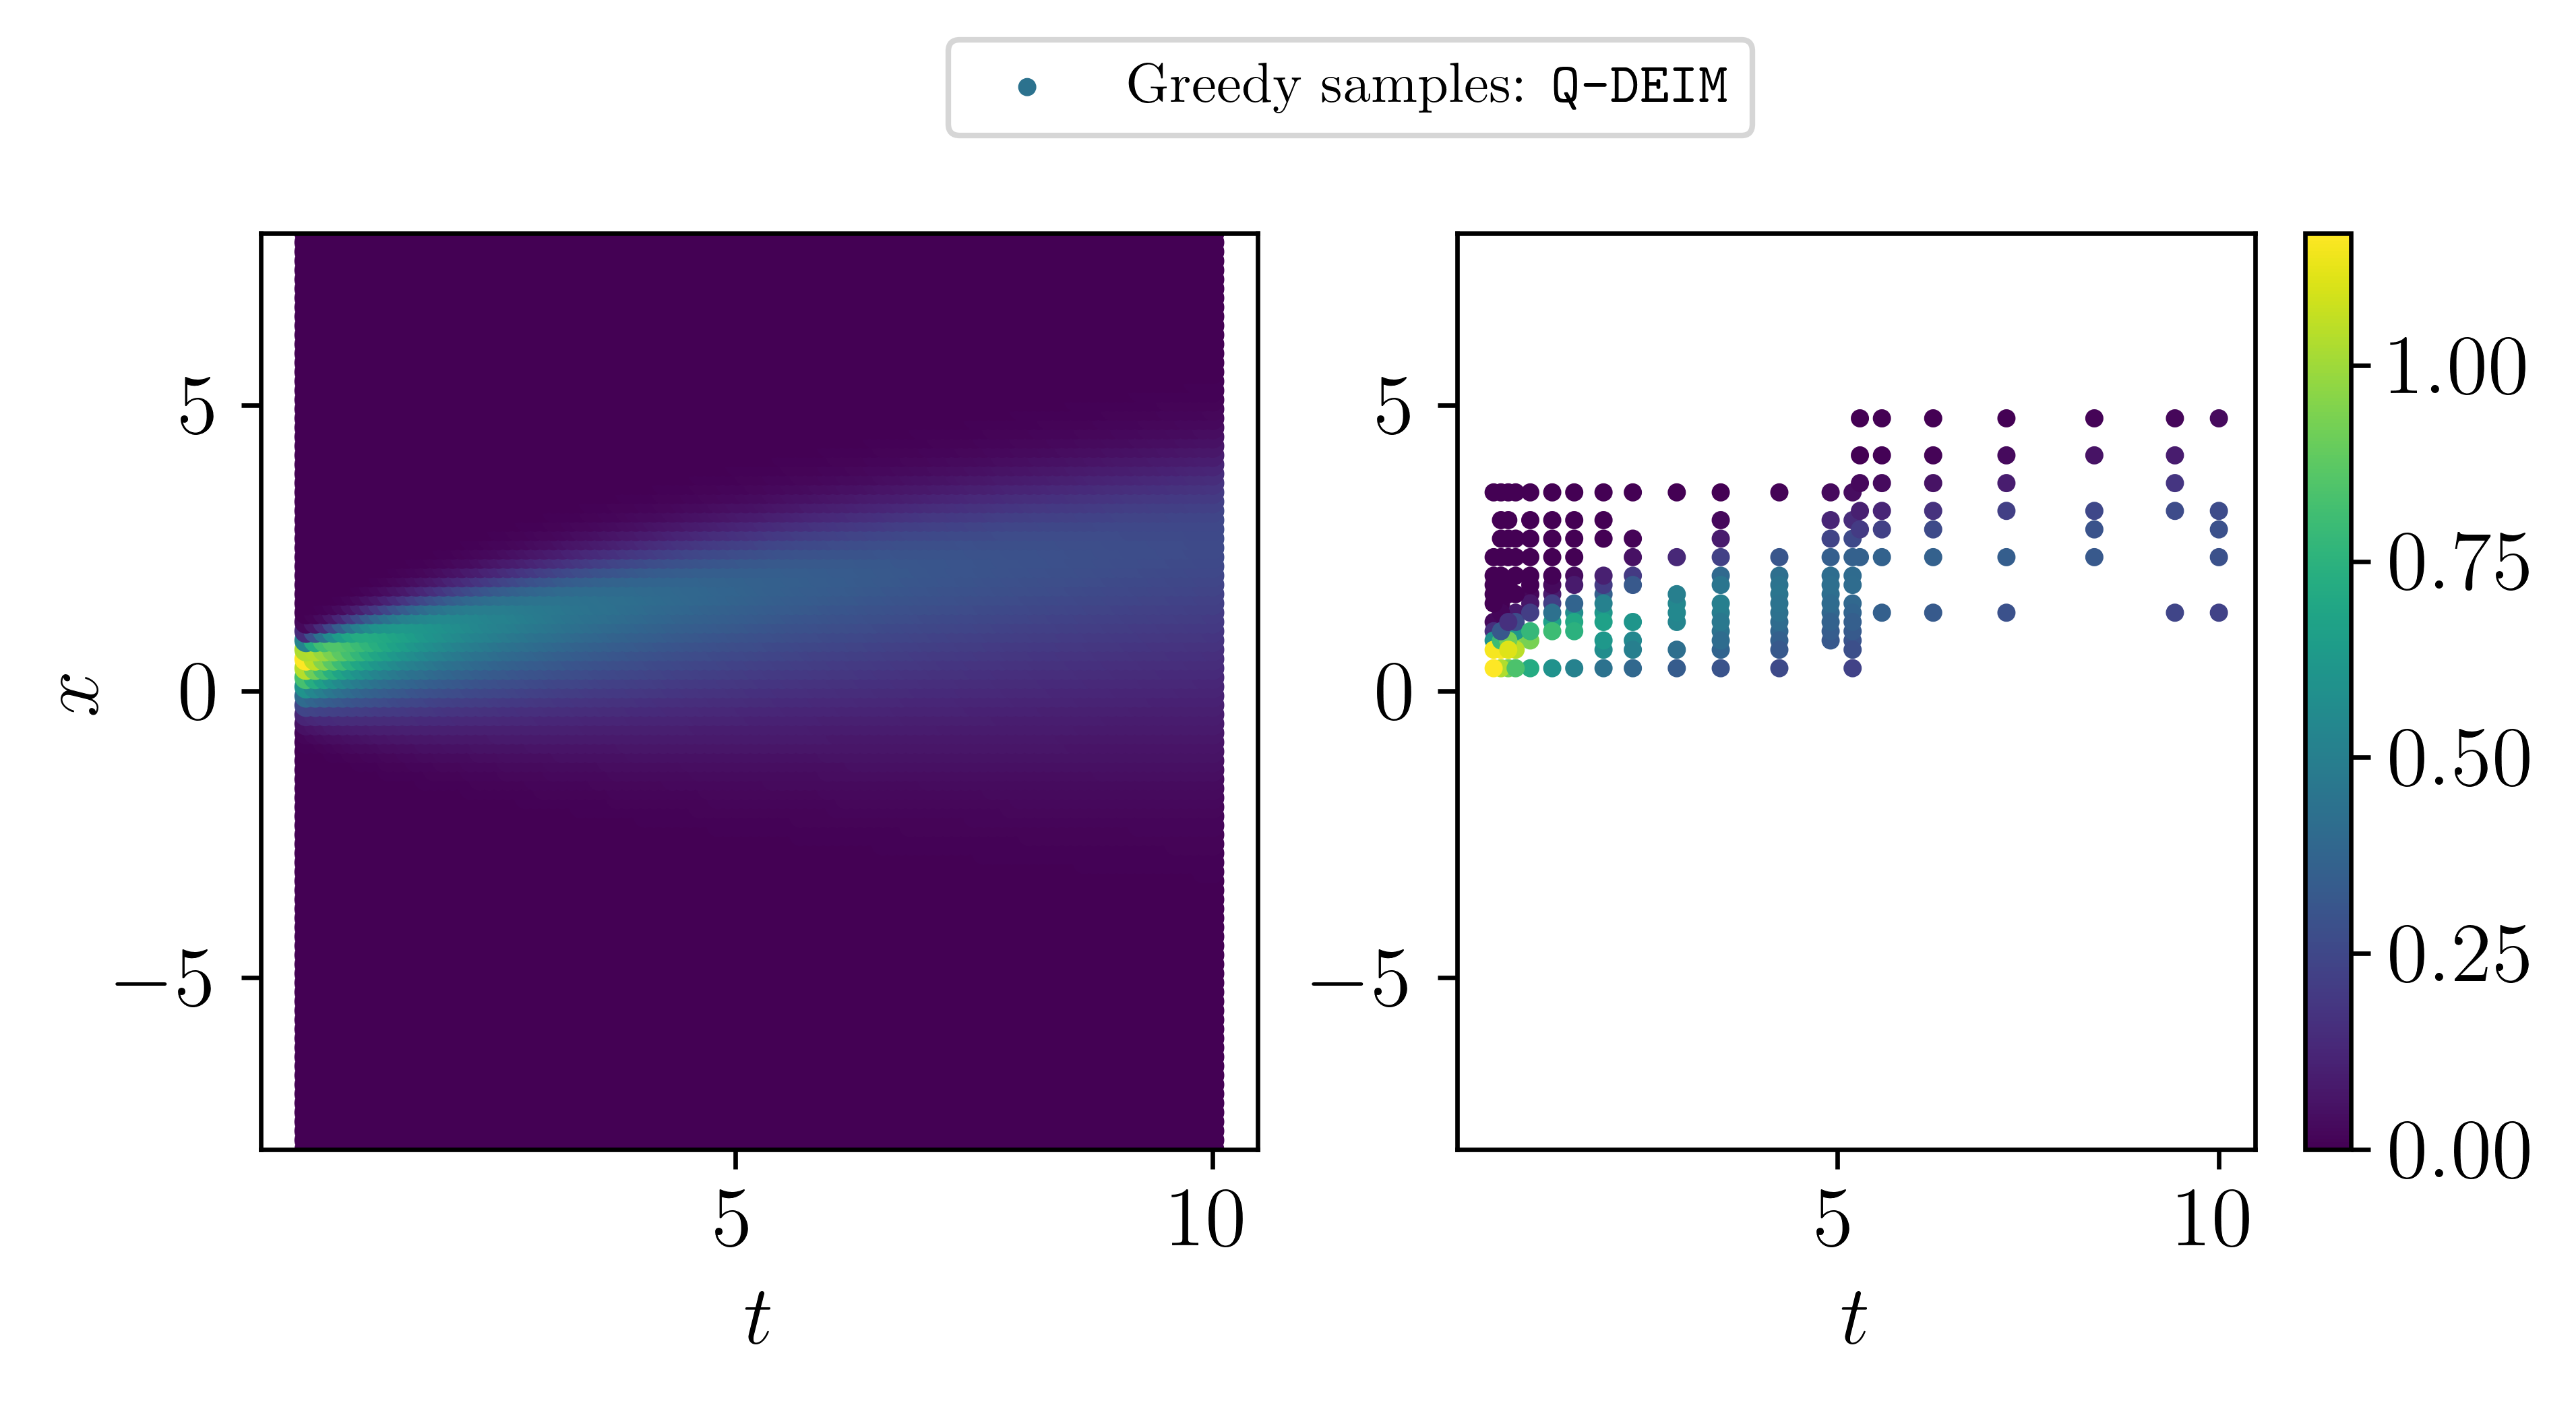
\includegraphics[trim = 0cm 0.cm 0.cm 0cm, clip, height = 6.5cm]{./Burgers_DEIM_schematic_200_poly_order_ 2_diff_order_ 3.png}
		\end{tabular}};
		% Implicit part
		\node[ fill = white,draw = green!50!black,  right = 1cm of burger.east, text = black, thick,rounded corners = 0.5ex, anchor=west,] (implicit_respresentation) {
			\begin{tabular}{c}
%				{\color{red!30!black} \huge Identify simultaneously implicit respresentation and neural dynamics} \\[5pt]
				%	\includegraphics[scale = 1.0]{Implicit_respresentation.pdf}
				{\color{red!30!black} \huge Network for implicit representation} \\[5pt]
				\begin{tikzpicture}[cir/.style={circle,draw=#1,minimum size=0.5},y=1cm,font=\sffamily, inner sep=7,transform shape,scale=1.0]
					\begin{scope}[rotate=0, scale = 0.8]
						\draw[draw=\fillcolor, opacity=0.4, thick, rounded corners=.1cm, fill = cyan!10!white ] (-0.75,-4.8) rectangle ++(8,5.4);
						%%
						\node[cir=black,fill=cyan!50!black, draw = \boundarycolor, ultra thick] (I1) at (-2,-1.5) {};
						\node[cir=black,fill=cyan!50!black,draw = \boundarycolor,ultra thick] (I2) at (-2,-3) {};
						%\node[cir=black,fill=cyan!50!black,draw = \boundarycolor,ultra thick] (I3) at (-2,-4.5) {};
						%%
						\node[cir=black,fill=\fillcolor, opacity=0.4,draw = \boundarycolor,ultra thick] (a1) at (0,0) {};
						\node[cir=black,fill=\fillcolor, opacity=0.4,draw = \boundarycolor,ultra thick] (a2) at (0,-1) {};
						\node[cir=black,fill=\fillcolor, opacity=0.4,draw = \boundarycolor,ultra thick] (a3) at (0,-2) {};
						\node[cir=black,fill=\fillcolor, opacity=0.4,draw = \boundarycolor,ultra thick] (a4) at (0,-3) {};
						\node[cir=black,fill=\fillcolor, opacity=0.4,draw = \boundarycolor,ultra thick] (a5) at (0,-4) {};
						%%
						\node[cir=cyan!50!black,fill=\fillcolor, opacity=0.4,draw = \boundarycolor,ultra thick] (b1) at (2,0) {};
						\node[cir=cyan!50!black,fill=\fillcolor, opacity=0.4,draw = \boundarycolor,ultra thick] (b2) at (2,-1) {};
						\node[cir=cyan!50!black,fill=\fillcolor, opacity=0.4,draw = \boundarycolor,ultra thick] (b3) at (2,-2) {};
						\node[cir=cyan!50!black,fill=\fillcolor, opacity=0.4,draw = \boundarycolor,ultra thick] (b4) at (2,-3) {};
						\node[cir=cyan!50!black,fill=\fillcolor, opacity=0.4,draw = \boundarycolor,ultra thick] (b5) at (2,-4) {};
						%%
						\node[cir=cyan!50!black,fill=\fillcolor, opacity=0.4,draw = \boundarycolor,ultra thick] (c1) at (4,0) {};
						\node[cir=cyan!50!black,fill=\fillcolor, opacity=0.4,draw = \boundarycolor,ultra thick] (c2) at (4,-1) {};
						\node[cir=cyan!50!black,fill=\fillcolor, opacity=0.4,draw = \boundarycolor,ultra thick] (c3) at (4,-2) {};
						\node[cir=cyan!50!black,fill=\fillcolor, opacity=0.4,draw = \boundarycolor,ultra thick] (c4) at (4,-3) {};
						\node[cir=cyan!50!black,fill=\fillcolor, opacity=0.4,draw = \boundarycolor,ultra thick] (c5) at (4,-4) {};
						%%
						\node[cir=cyan!50!black,fill=\fillcolor, opacity=0.4,draw = \boundarycolor,ultra thick] (d1) at (6,0) {};
						\node[cir=\boundarycolor,fill=\fillcolor, opacity=0.4,draw = \boundarycolor,ultra thick] (d2) at (6,-1) {};
						\node[cir=\boundarycolor,fill=\fillcolor, opacity=0.4,draw = \boundarycolor,ultra thick] (d3) at (6,-2) {};
						\node[cir=\boundarycolor,fill=\fillcolor, opacity=0.4,draw = \boundarycolor,ultra thick] (d4) at (6,-3) {};
						\node[cir=\boundarycolor,fill=\fillcolor, opacity=0.4,draw = \boundarycolor,ultra thick] (d5) at (6,-4) {};
						%%
						\node[cir=black,fill=green!50!red, draw = \boundarycolor,ultra thick] (O1) at (8,-2) {};
						%\node[cir=black,fill=green!50!red, draw = \boundarycolor,ultra thick] (O2) at (8,-1.0) {};
						
						
						\foreach \i/\j in {a/b,c/d} {
							\foreach \cnto in {1,2,3,4,5} {
								\foreach \cntt in {1,2,3,4,5} {
									\draw[thick] (\i\cnto.east)--(\j\cntt.west);
								}
							}
						}
						
						\foreach \i/\j in {I/a} {
							\foreach \cnto in {1,2} {
								\foreach \cntt in {1,2,3,4,5} {
									\draw[thick] (\i\cnto.east)--(\j\cntt.west);
								}
							}
						}
						
						\foreach \i/\j in {d/O} {
							\foreach \cnto in {1,2,3,4,5} {
								\foreach \cntt in {1} {
									\draw[thick] (\i\cnto.east)--(\j\cntt.west);
								}
							}
						}
						
						\draw[decorate sep={1mm}{2.5mm},fill] (3.1,-0.07) -- (3.8,-0.07);
						\draw[decorate sep={1mm}{2.5mm},fill] (3.1,-1.0) -- (3.8,-1.0);
						\draw[decorate sep={1mm}{2.5mm},fill] (3.1,-2.0) -- (3.8,-2.0);
						\draw[decorate sep={1mm}{2.5mm},fill] (3.1,-3.0) -- (3.8,-3.0);
						\draw[decorate sep={1mm}{2.5mm},fill] (3.1,-4.0) -- (3.8,-4.0);		
					\end{scope}
					
					\draw (I1) node[blue!50!\boundarycolor,left=0.15cm] { \Large $t_i$};
					\draw (I2) node[blue!50!\boundarycolor,left=0.15cm] { \Large $x_i$};
					%\draw (I3) node[blue!50!\boundarycolor,left=0.15cm] { \Large $y_{2,0}^{[j]}$};
					%					\draw (I2) node[blue!50!\boundarycolor,below=0.15cm] { \Large $\mathbf x$};
					\draw (O1) node[blue!50!\boundarycolor, right=0.01cm] {\hspace{0.2cm} \Large $ \hat{u}$};
					%\draw (O2) node[blue!50!\boundarycolor,right=0.01cm] {\hspace{0.2cm} \Large $ \hat{x}_1$};
					\node (n1) [fill=blue!25,draw=black, below right = -0.74cm and +0.11cm of b3, opacity=0.75] {\Large $ \mathcal{G}_\theta $};     
				\end{tikzpicture}\\[10pt]
				{\color{red!30!black} \huge~~~~ } \\[5pt]
				%
				%%%%%%%%%%%%%%%%%%%%%%%%%%%%%%%%%%%%%%%%
				%%%%%%%%%%%%%%%%%%%%%%%%%%%%%%%%%%%%%%%%
				
%				
%				\begin{tikzpicture}[cir/.style={circle,draw=#1,minimum size=0.5},y=1cm,font=\sffamily, inner sep=7,transform shape,scale=1.0]
%				\begin{scope}[rotate=0, scale = 0.8]
%				\draw [\fillcolorgreen, thick] (0,0) to [square left brace ] (0,4.4);
%				\draw[draw=\fillcolorgreen, thick, rounded corners=.1cm, fill = green!10!white ] (0.0,0.2) rectangle ++(0.2,3.5);
%				\draw[draw=\fillcolorgreen, thick, rounded corners=.1cm, fill = green!10!white ] (0.5,0.2) rectangle ++(0.2,3.5);
%				\draw [\fillcolorgreen, thick] (0.8,0) to [square right brace ] (0.8,4.4);
%				\node [] at (1.2,2) (eq) {\Huge =};
%				\draw [\fillcoloblue, thick] (2.75,0) to [square left brace ] (2.75,4.4);
%				\draw[draw=\fillcoloblue, thick, rounded corners=.1cm, fill = green!10!white ] (2.75,0.2) rectangle ++(0.2,3.5);
%				\draw[draw=\fillcoloblue, thick, rounded corners=.1cm, fill = green!10!white ] (3.25,0.2) rectangle ++(0.2,3.5);
%				\draw[draw=\fillcoloblue, thick, rounded corners=.1cm, fill = green!10!white ] (3.75,0.2) rectangle ++(0.2,3.5);
%				\node [] at (4.1,2) (eq) {\Huge $\cdots$};
%				\draw[draw=\fillcoloblue, thick, rounded corners=.1cm, fill = green!10!white ] (5.75,0.2) rectangle ++(0.2,3.5);
%				\draw [\fillcoloblue, thick] (6.05,0) to [square right brace ] (6.05,4.4);
%				\draw [\fillcolor, thick] (7.2,-1.2) to [square left brace ] (7.2,4.4);
%				\draw[draw=\fillcolor, thick, rounded corners=.1cm, fill = green!10!white ] (7.2,-1.0) rectangle ++(0.2,4.7);
%				\draw[draw=\fillcolor, thick, rounded corners=.1cm, fill = green!10!white ] (7.7,-1.0) rectangle ++(0.2,4.7);
%				\draw [\fillcolor, thick] (8.0,-1.2) to [square right brace ] (8.0,4.4);
%				\node [] at (-0.3,4.0) (dx1) {\Large $\dot x_1$};
%				\node [] at (0.2,4.0) (dx1) {\Large $\dot x_2$};
%				\node [] at (2.45,4.0) (dx1) {\Large $1$};
%				\node [] at (2.95,4.0) (dx1) {\Large $u_x$};
%				\node [] at (3.45,4.0) (dx1) {\Large $u_{xx}$};
%				\node [] at (5.4,4.0) (dx1) {\Large $x_2^4$};
%				\node [] at (6.8,4.0) (dx1) {\Large $\xi_1$};
%				\node [] at (7.3,4.0) (dx1) {\Large $\xi_2$};
%				\end{scope}
%				\end{tikzpicture}
				
				
				%%%%%%%%%%%%%%%%%%%%%%%%%%%%%%%%%%%%%%%%%
				%%%%%%%%%%%%%%%%%%%%%%%%%%%%%%%%%%%%%%%%%
				
%					{\color{red!30!black} \huge Find implicit respresentation of data} \\[5pt]
				%	\includegraphics[scale = 1.0]{Implicit_respresentation.pdf}
				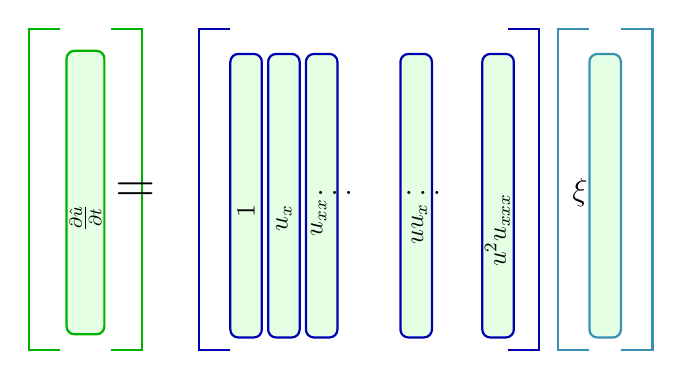
\begin{tikzpicture}[cir/.style={circle,draw=#1,minimum size=0.5},y=1cm,font=\sffamily, inner sep=7,transform shape,scale=1.0]
				\begin{scope}[rotate=0, scale = 0.8]
				% Simple brace

    		    \draw [\fillcolorgreen, thick] (-2,0) to [square left brace ] (-2, 5.1);
				\draw[draw=\fillcolorgreen, thick, rounded corners=.1cm, fill = green!10!white ] (-1.9,0.25) rectangle ++(0.6,4.5);
				%\draw[draw=\fillcolorgreen, thick, rounded corners=.1cm, fill = green!10!white ] (0.5,0.2) rectangle ++(0.2,3.5);
    		    \draw [\fillcolorgreen, thick] (-1.2,0) to [square right brace ] (-1.2, 5.1);
    		    \node [] at (-0.8,2.5) (eq) {\Huge =};
    		    
				\draw [\fillcoloblue, thick] (0.7, 0) to [square left brace ] (0.7, 5.1);
				\draw[draw=\fillcoloblue, thick, rounded corners=.1cm, fill = green!10!white ] (0.7,0.2) rectangle ++(0.5,4.5);
				\draw[draw=\fillcoloblue, thick, rounded corners=.1cm, fill = green!10!white ] (1.3,0.2) rectangle ++(0.5,4.5);
				\draw[draw=\fillcoloblue, thick, rounded corners=.1cm, fill = green!10!white ] (1.9,0.2) rectangle ++(0.5,4.5);
				\node [] at (2.4,2.5) (eq) {\Large $\dots$};
				\draw[draw=\fillcoloblue, thick, rounded corners=.1cm, fill = green!10!white ] (3.4,0.2) rectangle ++(0.5,4.5);
				\node [] at (3.8, 2.5) (eq) {\Large $\dots$};
				\draw[draw=\fillcoloblue, thick, rounded corners=.1cm, fill = green!10!white ] (4.7,0.2) rectangle ++(0.5,4.5);
    		     %\node [] at (4.1,2) (eq) {\Huge $\cdots$};
				%\draw[draw=\fillcoloblue, thick, rounded corners=.1cm, fill = green!10!white ] (5.75,0.2) rectangle ++(0.2,3.5);
				\draw [\fillcoloblue, thick] (5.1,0) to [square right brace ] (5.1,5.1);
				\draw [\fillcolor, thick] (6.4,0) to [square left brace ] (6.4,5.1);
				\draw[draw=\fillcolor, thick, rounded corners=.1cm, fill = green!10!white ] (6.4,0.2) rectangle ++(0.5,4.5);
				%\draw[draw=\fillcolor, thick, rounded corners=.1cm, fill = green!10!white ] (7.7,-1.0) rectangle ++(0.2,4.7);
				\draw [\fillcolor, thick] (6.9,0) to [square right brace ] (6.9, 5.1);
				
    		     \node [rotate=90] at (-1.6,2.10) (dx1) {\large $ \frac{\partial \hat{u} }{\partial t}$};
    		     %\node [] at (0.2,4.0) (dx1) {\Large $\dot x_2$};
    		     
    		    %\node [rotate=90] at (2.45,4.0) (dx1) {\Large $u$};
				\node [rotate=90] at (0.95,2.2) (dx1) {\large $1$};
				\node [rotate=90] at (1.55,2.1) (dx1) {\large $u_{x}$};
				\node [rotate=90] at (2.1,2.1) (dx1) {\large $u_{xx}$};
				\node [rotate=90] at (3.7,2.0) (dx1) {\large $u u_{x}$};
				\node [rotate=90] at (4.94,1.9) (dx1) {\large $u^2 u_{xxx}$};
				\node [] at (6.25, 2.5) (dx1) {\Large $\xi$};
				%\node [] at (6.1,1) (dx1) {\Large $p_2$};
				%\node [] at (6.1,3) (dx1) {\Large $p_1$};
				%\node [] at (30.1,8) (dx1) {\Huge $\xi$};
				\end{scope}
				
				\end{tikzpicture}
				%%%%%%%%%%%%%%%%%%%%%%%%%%%%%%%%%%%%%%%%%%
			\end{tabular}
		};
		%%%%%%%%%%%%
		% RK part
%		\node[ fill = white,draw = green!50!black,  below right = 0cm and 8.5cm of implicit_respresentation.north, text = black, thick,rounded corners = 0.5ex, rotate = 0] (RKsteps) {
%			\begin{tabular}{c}
%				{\color{red!30!black} \huge Intergral constraint} \\[5pt]
%				%		\includegraphics[trim = 0cm 1.0cm 0cm 0.25cm, clip, scale = 0.4, angle = 0]{RK4_Steps.pdf}
%				$\mathbf x(t_j) \approx \mathbf x(t_i) + \int_{t_i}^{t_j}\mathbf g(\mathbf x(\tau))d\tau $
%				\vspace{-0.75cm}
%			\end{tabular}
%		};
		
		\node [] at (0,-4.0) [ fill = none,draw = green!50!black,below = 2.0cm of implicit_respresentation.south, thick,rounded corners = 0.5ex, minimum width = .5cm, minimum height = .5cm] (loss) {\Large
			\begin{tabular}{c}
				{\color{red!50!black} \huge Objective (loss) function} \\
				\vspace{0.2cm}
				
%				$
%				\mathbf{\mathcal{L}} =  \frac{\mu_1}{\mathcal{N}_t \cdot \mathcal{N}}\sum_{j=1}^{\mathcal{N}_t} \sum_{k=1}^{\mathcal{N}}\Big\|{\mathbf{x}^{[j]}(t_k) - \hat{\mathbf{x}}^{[j]}(t_k)}\Big\|_2^2 +
%				\frac{\mu_2}{\mathcal{N}_t \cdot \mathcal{N}}
%				\sum_{j=1}^{\mathcal{N}_t} \sum_{k=1}^{\mathcal{N}} \Big\| \Theta\big(\hat{\mathbf{x}}^{[j]}(t_k)\big) \hat{\Xi} -
%				\dot{\hat{\mathbf{x}}}(t_k) \Big\|_2^2$\\$+
%				\frac{\mu_3}{h} \frac{1}{\mathcal{N}_t \cdot \mathcal{N}}\sum_{j=1}^{\mathcal{N}_t} \sum_{k=1}^{\mathcal{N}} \Big\| \hat{\mathbf{x}}^{[j]}(t_k) - \hat{\mathbf{x}}^{[j]}_{RK4}(t_k) \Big\|_2^2
%				$\\
				
%				$
%				\mathbf{\mathcal{L}} =  
%				\sum_{j=1}^{\mathcal{N}_t} \sum_{k=1}^{\mathcal{N}}\Bigg( \frac{\mu_1}{\mathcal{N}_t \cdot \mathcal{N}}  \Big\|{\mathbf{x}^{[j]}(t_k) - \hat{\mathbf{x}}^{[j]}(t_k)}\Big\|_2^2 +
%				\frac{\mu_2}{\mathcal{N}_t \cdot \mathcal{N}}
%				 \Big\| \Theta\big(\hat{\mathbf{x}}^{[j]}(t_k)\big) \hat{\Xi} -
%				\dot{\hat{\mathbf{x}}}(t_k) \Big\|_2^2+
%				\frac{\mu_3}{h} \frac{1}{\mathcal{N}_t \cdot \mathcal{N}} \Big\| \hat{\mathbf{x}}^{[j]}(t_k) - \hat{\mathbf{x}}^{[j]}_{RK4}(t_k) \Big\|_2^2 \Bigg)
%				$\\
				
				
				\\
				
				$
				\mathbf{\mathcal{L}} = \frac{1}{\mathcal{N} }
				\sum_{i=1}^{\mathcal{N}  } \Big( \mathbf{u}(t_i,x_i) - \hat{\mathbf{u}}(t_i,x_i) \Big)^2 + \frac{1}{\mathcal{N}} \sum_{i=1}^{\mathcal{N}} \Big( \frac{\partial \hat{\mathbf{u}}  (t_i,x_i) } {\partial t_i} - \mathbf{\Theta}\big( \hat{\mathbf{u}}(t_i,x_i) \big) (\xi \cdot \texttt{g}) \Big)^2,
				$
				
				%$
				%\text{s. t.}\ \ \
				%\mathbf{Q} \mathbf{R}  = %\mathbf{\Theta}(\hat{\mathbf{U}}),\ \hat{p} = %\mathbf{R}^{-1} \mathbf{Q}^\top \hat{\mathbf{U}}_t.
				%$
				\vspace{0.2cm}
%				$
%				\mathbf{\mathcal{L}}_{\texttt{MSE}} = \frac{1}{\mathcal{N}_t \cdot \mathcal{N}}\sum_{j=1}^{\mathcal{N}_t} \sum_{k=1}^{\mathcal{N}}\Big\|{\mathbf{x}^{[j]}(t_k) - \hat{\mathbf{x}}^{[j]}(t_k)}\Big\|_2^2,$\\$
%				\mathbf{\mathcal{L}}_{\texttt{deri}} = \frac{1}{\mathcal{N}_t \cdot \mathcal{N}}
%				\sum_{j=1}^{\mathcal{N}_t} \sum_{k=1}^{\mathcal{N}} \Big\| \Theta\big(\hat{\mathbf{x}}^{[j]}(t_k)\big) \hat{\Xi} -
%				\dot{\hat{\mathbf{x}}}(t_k) \Big\|_2^2,$\\$
%				\mathbf{\mathcal{L}}_{RK4} = \frac{1}{h} \frac{1}{\mathcal{N}_t \cdot \mathcal{N}}\sum_{j=1}^{\mathcal{N}_t} \sum_{k=1}^{\mathcal{N}} \Big\| \hat{\mathbf{x}}^{[j]}(t_k) - \hat{\mathbf{x}}^{[j]}_{RK4}(t_k) \Big\|_2^2.
%				$
			\end{tabular}
		};
		
			\node[ fill = white,draw = green!50!black,  right =1.15cm  of implicit_respresentation.east, text = black, thick,rounded corners = 0.5ex, minimum height=4cm] (denoised) {
%		\begin{tabular}[t]{c}
%			{\color{red!30!black} \huge   governing equation  ~~~~~~~~} \\[5pt]
%			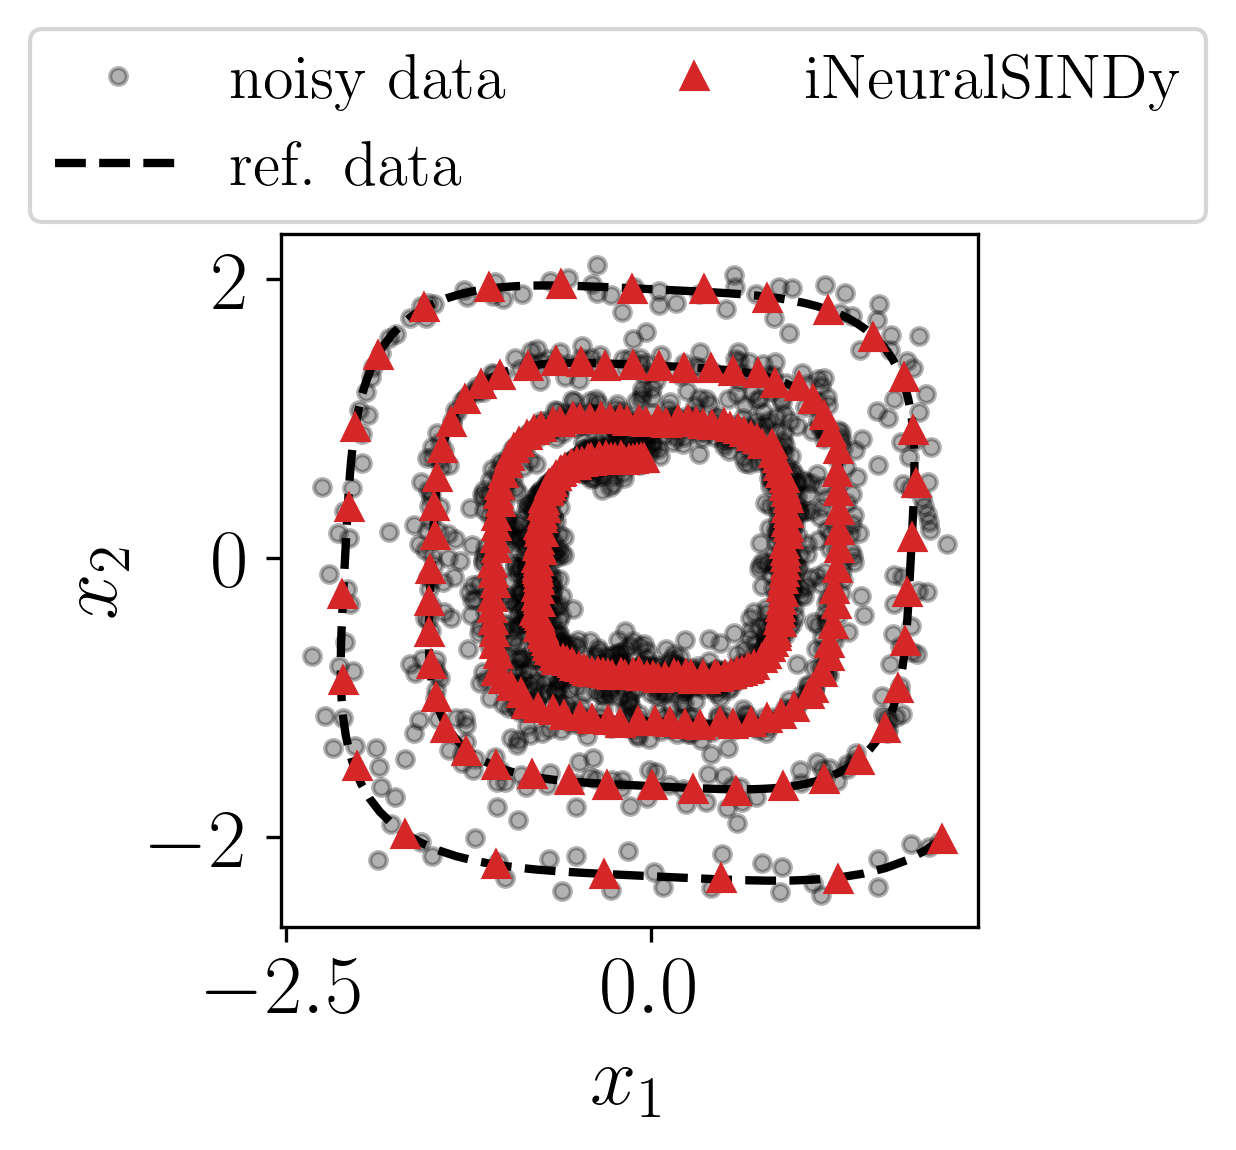
\includegraphics[trim = 0cm 0cm 0cm 0cm, clip, width=7cm]{./Cubic_Oscilator_noise_0.0_estimated_model_0.05.png}  \\
%		\end{tabular}
%		\quad
%		\begin{tabular}{rr}
%			0.00 & 0.00 \\
%			0.00 & 0.00  \\
%			$0.00$ & $0.00$ \\
%			$0.00$ & $0.00$ \\
%			$0.00$ & $0.00$ \\
%			$0.00$ & $0.00$ \\
%			$-0.10$ & $-2.00$ \\
%			$0.00$ & $0.00$ \\
%			$0.00$ & $0.00$ \\
%			$2.00$ & $-0.10 $
%		\end{tabular}

	
		\begin{tabular}{c}
			
			\begin{tabular}{c}
				{\color{red!30!black}\huge~~~~~~~~~~~~~~Learned coefficient vector} \\[5pt]
				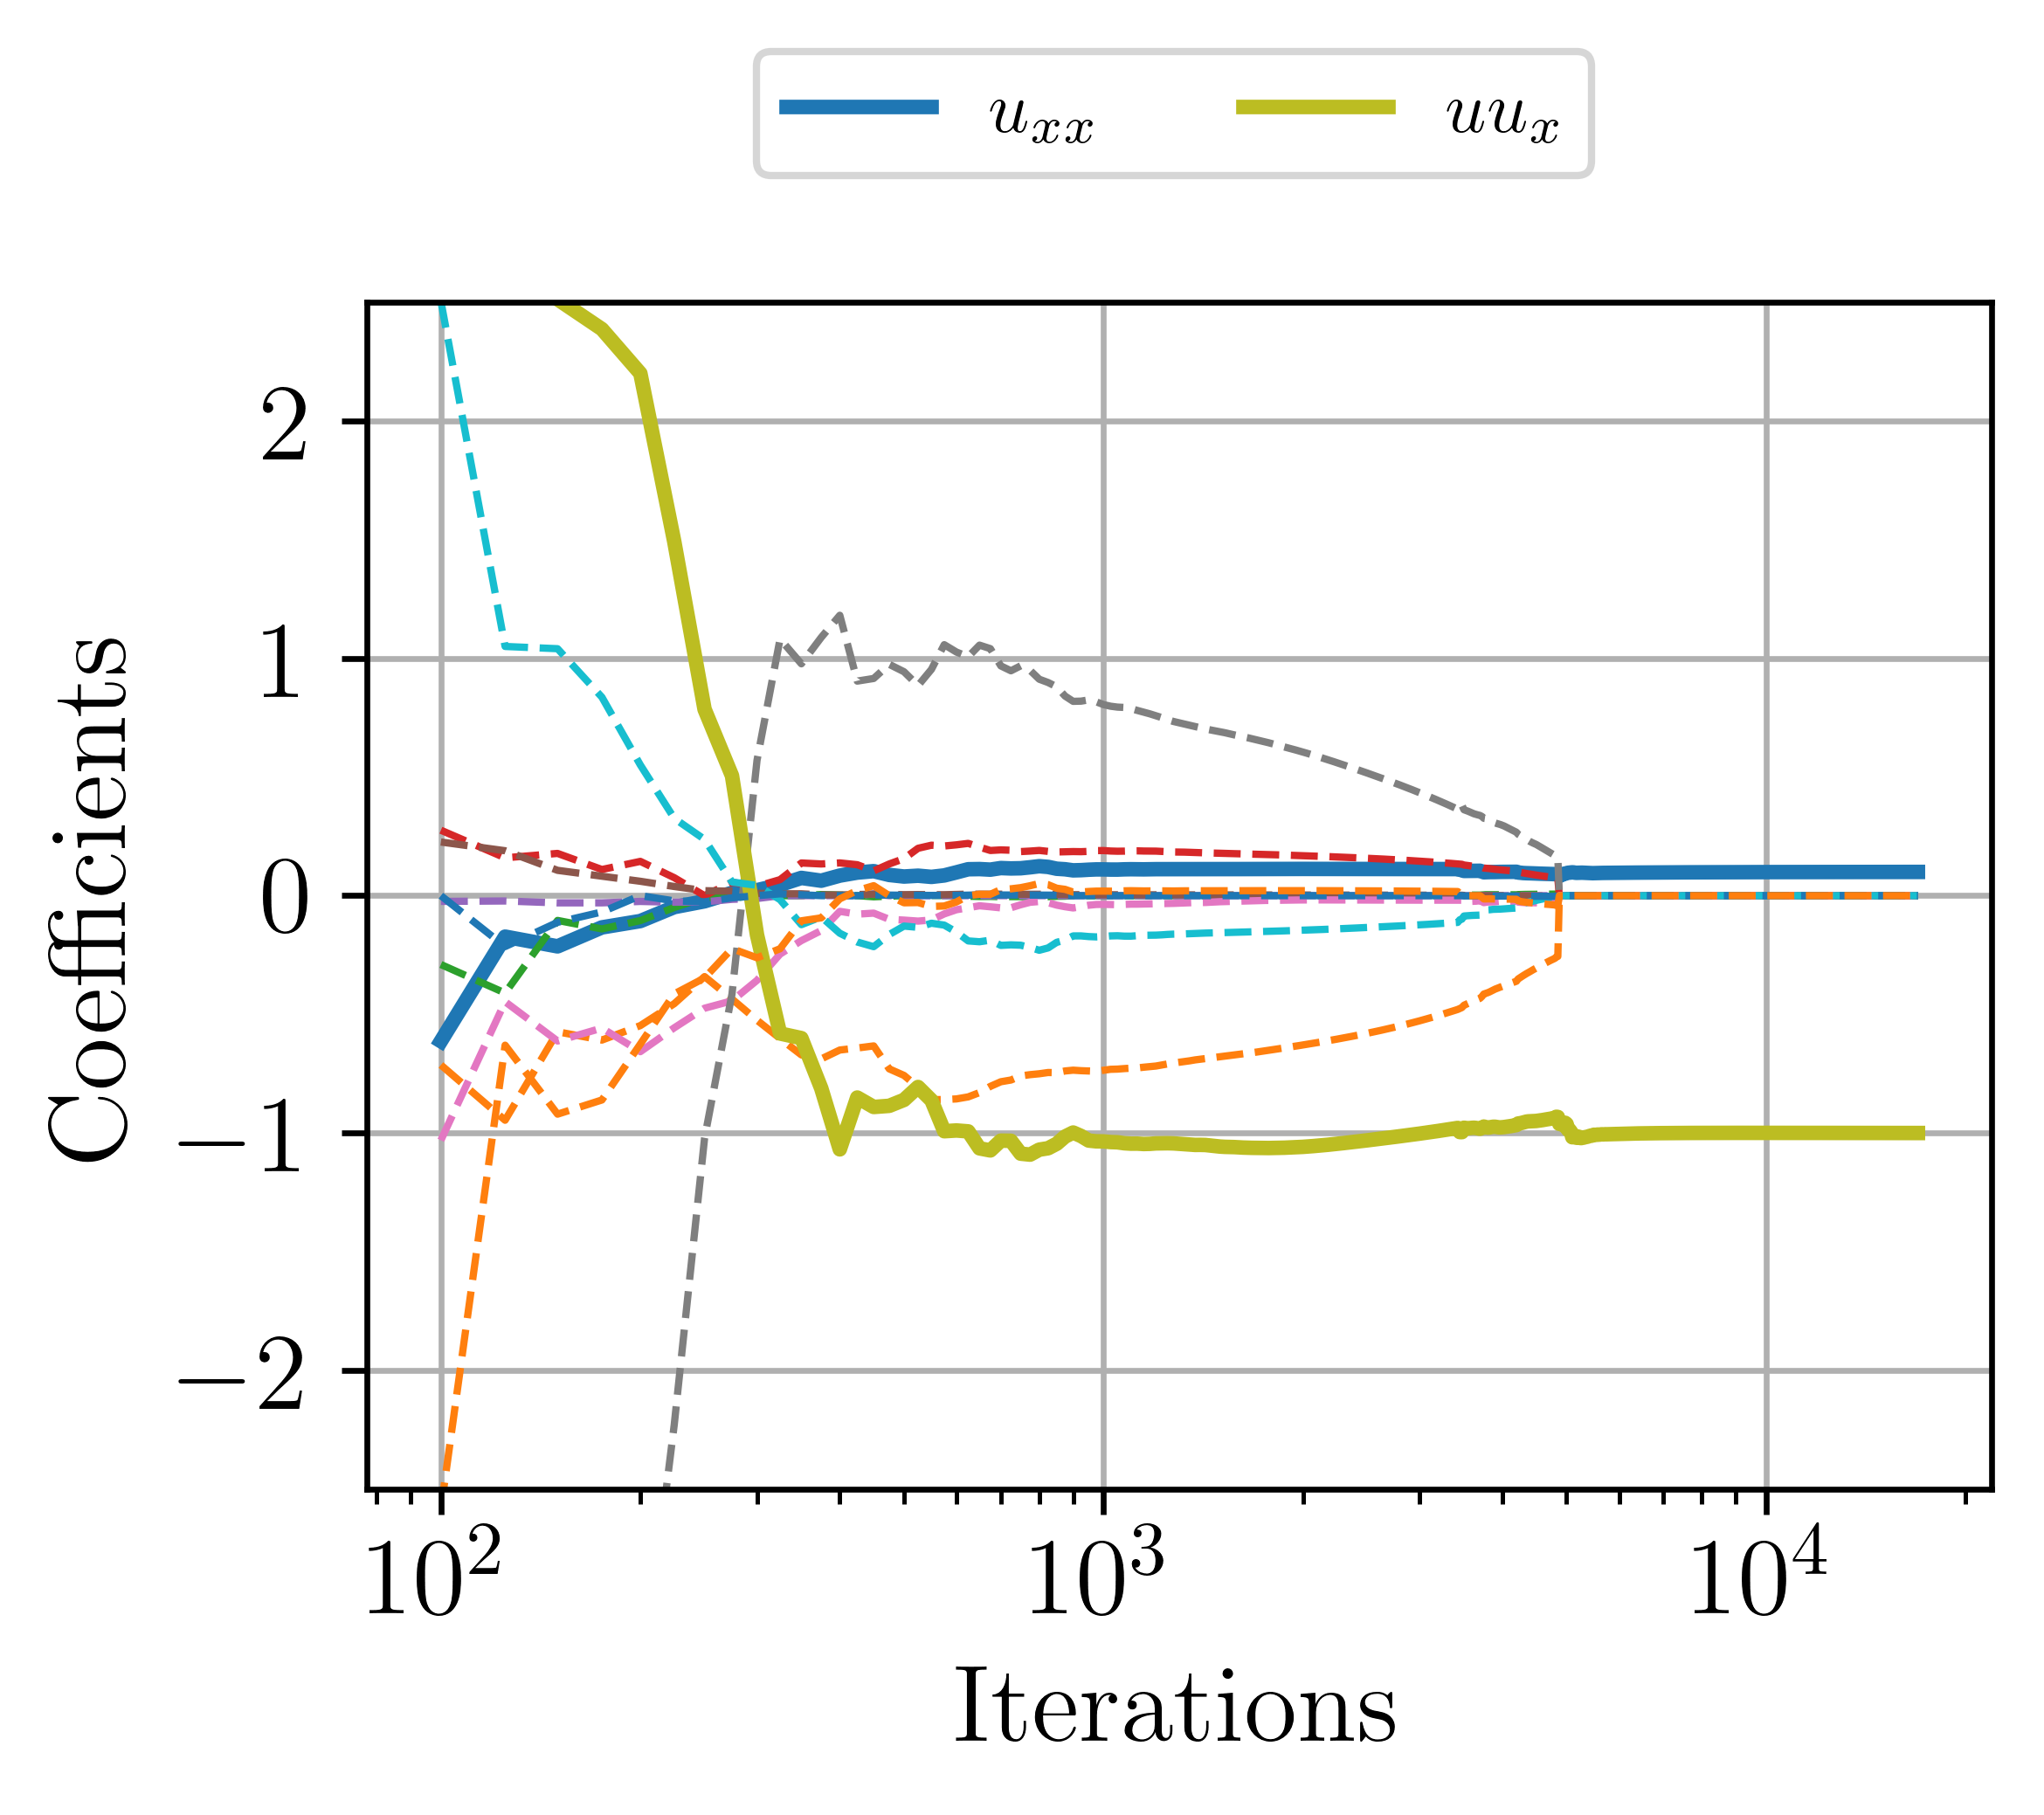
\includegraphics[trim=0cm 0cm 0cm 0cm, clip, width=9cm]{./Burgers_coeff_iterations_DEIM_200_poly_order_ 2_diff_order_ 3.png}
			\end{tabular}\hspace{-0.5cm}
			
			\begin{tabular}{c}
				
				
				
				
				
				
%				\centering
%				$\Theta = 
%				\begin{bmatrix}
%				1\\
%				u_x
%				\\
%				u_{xx}\\
%				u_{xxx}\\
%				u\\
%				u u_x\\
%				u u_{xx}\\
%				u u_{xxx}\\
%				u^2\\
%				u^2 u_x\\
%				u^2 u_{xx}\\
%				u^2 u_{xxx}
%				\end{bmatrix}^\top$
%				
%				
%				$\xi=
%				\begin{bmatrix}
%				0.000\\
%				0.000\\
%				0.100\\
%				0.000\\
%				0.000\\
%				-0.999\\
%				0.000\\
%				0.000\\
%				0.000\\
%				0.000\\
%				0.000\\
%				0.000\\
%				\end{bmatrix}
%				$
				
				
				$\begin{bmatrix}
				\Theta \\
				\begin{tabular}{c}
					-\ -\ -\ -\ -	
					\\
					$1$\\
					$u_x$\\
					$u_{xx}$\\
					$u_{xxx}$\\
					$u$\\
					$u u_x$\\
					$u u_{xx}$\\
					$u u_{xxx}$\\
					$u^2$\\
					$u^2 u_x$\\
					$u^2 u_{xx}$\\
					$u^2 u_{xxx}$
				\end{tabular}
				\end{bmatrix}
				$
				
				
				
				
				$\begin{bmatrix}
				\xi\\
				\begin{tabular}{r}
				-\ -\ -\ -\ -
				\\
				0.000\\
				0.000\\
				0.100\\
				0.000\\
				0.000\\
				-0.999\\
				0.000\\
				0.000\\
				0.000\\
				0.000\\
				0.000\\
				0.000\\
				\end{tabular}
				\end{bmatrix}
				$
				
			
				
			\end{tabular}

		\end{tabular}
		};
		  %\draw [\fillcolorgreen, thick] ($(denoised.south) + (3.7,1.8)$) to [square left brace ] ($(denoised.south) + (3.7,7.1)$) ;
%		  \node [] at ($(denoised.south) + (-0.1,-5)$)  {\large \begin{tabular}{c}
%		  		1 \\ $x_1 $ \\ $x_2$ \\ 
%		  		$x_1^2$ \\
%		  		$x_1 x_2$\\
%		  		$x_2^2$\\
%		  		$x_1^3$\\
%		  		$x_1^2 x_2$\\
%		  		$x_1 x^2_2$\\
%		  		$x^3_2$     
%		  \end{tabular}};
		  %\draw [\fillcolorgreen, thick] ($(denoised.south) + (3.95,1.8)$) to [square right brace ] ($(denoised.south) + (3.95,7.1)$) ;
		
		  %\draw [\fillcolorgreen, thick] ($(denoised.south) + (5.4,1.8)$) to [square left brace ] ($(denoised.south) + (5.4,7.1)$) ;
		  
		  %\node [] at ($(denoised.south) + (4.1,-2.5)$) {\large
		  %\begin{tabular}{rr}
		 % 	$\ \ \xi_1\ \ \ $ & $\ \xi_2\ \ $\\
	  	%\end{tabular}};
	  			  
  		
		  
%		\node [] at ($(denoised.south) + (4,-5)$)  {\small \begin{tabular}{rr}
%				0.00 & 0.00 \\
%				0.00 & 0.00  \\
%				$0.00$ & $0.00$ \\
%				$0.00$ & $0.00$ \\
%				$0.00$ & $0.00$ \\
%				$0.00$ & $0.00$ \\
%				$-0.10$ & $-2.00$ \\
%				$0.00$ & $0.00$ \\
%				$0.00$ & $0.00$ \\
%				$2.00$ & $-0.10 $
%		\end{tabular}};
	
		%\draw [\fillcolorgreen, thick] ($(denoised.south) + (6.9,1.8)$) to [square right brace ] ($(denoised.south) + (6.9,7.1)$) ;

		\node[ fill = none,draw = none,right =  -0.5cm  of burger.east, thick,rounded corners = 0.5ex, minimum width = .5cm, minimum height = .5cm] (arrow1) {
			\tikzfancyarrow[1.3cm]{{\Large ~~Data~~~}}
		};
	
				\node[ fill = none,draw = none,  right =  -0.8cm  of implicit_respresentation.east, thick,rounded corners = 0.5ex, minimum width = .5cm, minimum height = .5cm, rotate=0] (arrow2) {
			\tikzfancyarrow[1.3cm]{{\rotatebox{0}{\Large Learned}}}
		};
				\node[ fill = none,draw = none, above left =  -1.25cm and -3.5cm  of loss.north, thick,rounded corners = 0.5ex, minimum width = 0.5cm, minimum height = .5cm, rotate=-90, opacity=0.75] (arrow3) {
			\tikzfancyarrowsecond[1.3cm]{{\rotatebox{00}{\Large \begin{tabular}[t]{l} Optimizing \\ parameters \end{tabular}}}}
		};

	\node[ fill = green!10!white,draw = green!50!black, below right =  -0.8cm and -0.35cm  of burger.north, thick,rounded corners = 0.5ex, minimum width = .5cm, minimum height = .5cm] (a) {\Huge a};
		\node[ fill = green!10!white,draw = green!50!black, below right =  -1.05cm and 0.04cm  of implicit_respresentation.north, thick,rounded corners = 0.5ex, minimum width = .5cm, minimum height = .5cm] (b) {\Huge b};
		%
		%\node[ fill = green!10!white,draw = green!50!black, above right =  7.5cm and 0.25cm  of RKsteps.south, thick,rounded corners = 0.5ex, minimum width = .5cm, minimum height = .5cm] (c) {\Large c};
		%
		\node[ fill = green!10!white,draw = green!50!black, below right =  -0.8cm and -0.15cm  of loss.north, thick,rounded corners = 0.5ex, minimum width = .5cm, minimum height = .5cm] (c) {\Huge c};
		\node[ fill = green!10!white,draw = green!50!black, below right =  -1.cm and 0cm  of denoised.north, thick,rounded corners = 0.5ex, minimum width = .5cm, minimum height = .5cm] (d) {\Huge d};
	\end{tikzpicture}
\end{document}
